% Options for packages loaded elsewhere
\PassOptionsToPackage{unicode}{hyperref}
\PassOptionsToPackage{hyphens}{url}
\documentclass[
  11pt,
]{article}
\usepackage{xcolor}
\usepackage[left=3cm,right=5cm,top=2cm,bottom=2cm]{geometry}
\usepackage{amsmath,amssymb}
\setcounter{secnumdepth}{5}
\usepackage{iftex}
\ifPDFTeX
  \usepackage[T1]{fontenc}
  \usepackage[utf8]{inputenc}
  \usepackage{textcomp} % provide euro and other symbols
\else % if luatex or xetex
  \usepackage{unicode-math} % this also loads fontspec
  \defaultfontfeatures{Scale=MatchLowercase}
  \defaultfontfeatures[\rmfamily]{Ligatures=TeX,Scale=1}
\fi
\usepackage{lmodern}
\ifPDFTeX\else
  % xetex/luatex font selection
\fi
% Use upquote if available, for straight quotes in verbatim environments
\IfFileExists{upquote.sty}{\usepackage{upquote}}{}
\IfFileExists{microtype.sty}{% use microtype if available
  \usepackage[]{microtype}
  \UseMicrotypeSet[protrusion]{basicmath} % disable protrusion for tt fonts
}{}
\makeatletter
\@ifundefined{KOMAClassName}{% if non-KOMA class
  \IfFileExists{parskip.sty}{%
    \usepackage{parskip}
  }{% else
    \setlength{\parindent}{0pt}
    \setlength{\parskip}{6pt plus 2pt minus 1pt}}
}{% if KOMA class
  \KOMAoptions{parskip=half}}
\makeatother
\usepackage{longtable,booktabs,array}
\newcounter{none} % for unnumbered tables
\usepackage{calc} % for calculating minipage widths
% Correct order of tables after \paragraph or \subparagraph
\usepackage{etoolbox}
\makeatletter
\patchcmd\longtable{\par}{\if@noskipsec\mbox{}\fi\par}{}{}
\makeatother
% Allow footnotes in longtable head/foot
\IfFileExists{footnotehyper.sty}{\usepackage{footnotehyper}}{\usepackage{footnote}}
\makesavenoteenv{longtable}
\usepackage{graphicx}
\makeatletter
\newsavebox\pandoc@box
\newcommand*\pandocbounded[1]{% scales image to fit in text height/width
  \sbox\pandoc@box{#1}%
  \Gscale@div\@tempa{\textheight}{\dimexpr\ht\pandoc@box+\dp\pandoc@box\relax}%
  \Gscale@div\@tempb{\linewidth}{\wd\pandoc@box}%
  \ifdim\@tempb\p@<\@tempa\p@\let\@tempa\@tempb\fi% select the smaller of both
  \ifdim\@tempa\p@<\p@\scalebox{\@tempa}{\usebox\pandoc@box}%
  \else\usebox{\pandoc@box}%
  \fi%
}
% Set default figure placement to htbp
\def\fps@figure{htbp}
\makeatother
% definitions for citeproc citations
\NewDocumentCommand\citeproctext{}{}
\NewDocumentCommand\citeproc{mm}{%
  \begingroup\def\citeproctext{#2}\cite{#1}\endgroup}
\makeatletter
 % allow citations to break across lines
 \let\@cite@ofmt\@firstofone
 % avoid brackets around text for \cite:
 \def\@biblabel#1{}
 \def\@cite#1#2{{#1\if@tempswa , #2\fi}}
\makeatother
\newlength{\cslhangindent}
\setlength{\cslhangindent}{1.5em}
\newlength{\csllabelwidth}
\setlength{\csllabelwidth}{3em}
\newenvironment{CSLReferences}[2] % #1 hanging-indent, #2 entry-spacing
 {\begin{list}{}{%
  \setlength{\itemindent}{0pt}
  \setlength{\leftmargin}{0pt}
  \setlength{\parsep}{0pt}
  % turn on hanging indent if param 1 is 1
  \ifodd #1
   \setlength{\leftmargin}{\cslhangindent}
   \setlength{\itemindent}{-1\cslhangindent}
  \fi
  % set entry spacing
  \setlength{\itemsep}{#2\baselineskip}}}
 {\end{list}}
\usepackage{calc}
\newcommand{\CSLBlock}[1]{\hfill\break\parbox[t]{\linewidth}{\strut\ignorespaces#1\strut}}
\newcommand{\CSLLeftMargin}[1]{\parbox[t]{\csllabelwidth}{\strut#1\strut}}
\newcommand{\CSLRightInline}[1]{\parbox[t]{\linewidth - \csllabelwidth}{\strut#1\strut}}
\newcommand{\CSLIndent}[1]{\hspace{\cslhangindent}#1}
\setlength{\emergencystretch}{3em} % prevent overfull lines
\providecommand{\tightlist}{%
  \setlength{\itemsep}{0pt}\setlength{\parskip}{0pt}}
\usepackage{amsmath,amsfonts,amssymb}
\usepackage{booktabs}
\usepackage{float}
\DeclareMathOperator{\Var}{Var}
\DeclareMathOperator{\Cov}{Cov}
\DeclareMathOperator{\Corr}{Corr}
\usepackage{bookmark}
\IfFileExists{xurl.sty}{\usepackage{xurl}}{} % add URL line breaks if available
\urlstyle{same}
\hypersetup{
  pdftitle={Optimal Allocation of Observations across Run-In{,} Treatment{,} and Common Close Phases in Longitudinal Clinical Trials},
  pdfauthor={Ronald G. Thomas, Ph.D.},
  hidelinks,
  pdfcreator={LaTeX via pandoc}}

\title{Optimal Allocation of Observations across Run-In, Treatment, and
Common Close Phases in Longitudinal Clinical Trials}
\author{Ronald G. Thomas,
Ph.D.\thanks{Wertheim School of Public Health, UCSD; ORCID: 0000-0003-1686-4965}}
\date{May 11, 2026}

\begin{document}
\maketitle
\begin{abstract}
\textbf{Background.} Trial designers planning a longitudinal study with
a fixed total observation budget face an allocation question: how should
observations be distributed across run-in (\(J_0\)), treatment
(\(J_1\)), and common close (\(J_2\)) phases to minimise the variance of
the treatment-effect estimator? Existing guidance is heuristic; the
analytical optimum has not been previously characterised.

\textbf{Methods.} We formulate the allocation question as a discrete
optimisation problem over the Woodbury-based variance formula derived in
Paper 1 of this compendium. The solution is characterised as a function
of the signal-to-noise ratio \(\sigma_b / \sigma\). Extensions cover
three settings: non-equally-spaced designs in which the timing of
observations within each phase is also optimised; replicated endpoint
observations (closely spaced measurements at the end of treatment that
average out measurement error on the final assessment, analogous to
run-in averaging applied at the post-treatment end); and pattern-mixture
handling of dropout following the Frost-Kenward-Fox (2008) framework.

\textbf{Results.} The optimal allocation depends primarily on
\(\sigma_b / \sigma\). The common close phase is beneficial only when
this ratio exceeds a threshold that depends on \(J_1\); below the
threshold, all observations should go to the treatment phase.
Non-equally-spaced designs improve efficiency by 5-15\% over
equally-spaced designs at matched \(J\), with the largest gains at low
signal-to-noise ratios. Replicated endpoint observations reduce
measurement-error variance proportionally to their count, with
diminishing returns above 3-4 replicates.

\textbf{Conclusions.} The optimal-allocation rules derived here give
trial designers a closed-form decision procedure driven by the
signal-to-noise ratio. The procedure generalises to non-equally-spaced
and dropout-adjusted designs without sacrificing closed-form
tractability.
\end{abstract}

{
\setcounter{tocdepth}{2}
\tableofcontents
}
\section{Introduction}\label{introduction}

The relative efficiency surface in Paper 1 (Figure 1) demonstrates
diminishing returns from additional run-in observations: the first
run-in observation provides the largest variance reduction, while
subsequent observations contribute progressively less. Similarly, common
close observations improve efficiency but at a rate that depends on the
number of treatment observations \(J_1\).

These observations raise a design question that Paper 1 does not
address: given operational constraints on the total number of visits or
total trial duration, what is the optimal distribution of observations
across the three phases?

Winkens et al. (\citeproc{ref-winkens2005}{2005}) calculated optimal
time-point positions for linearly divergent treatment effects under
compound symmetry, but did not consider the run-in setting. Yi and
Panzarella (\citeproc{ref-yi2002}{2002}) derived sample sizes for trends
across repeated measurements under missing data. Frison and Pocock
(\citeproc{ref-frison1992}{1992}) showed that having more than one
pre-treatment measurement is beneficial for designs analyzed via ANCOVA.
Overall and Doyle (\citeproc{ref-overall1994}{1994}) provided sample
size formulas for repeated measurement designs. Galbraith and Marschner
(\citeproc{ref-galbraith2002}{2002}) developed general guidelines for
the design of clinical trials with longitudinal outcomes. The slopepower
command (\citeproc{ref-nash2021}{Nash et al. 2021}) and the longpower R
package (\citeproc{ref-iddi2022}{Iddi and Donohue 2022}) implement power
calculations for slope-comparison trials but do not optimize the
allocation of observations across phases.

\section{Problem formulation}\label{problem-formulation}

\subsection{Fixed total visits}\label{fixed-total-visits}

Given \(J\) total observations (excluding baseline), choose
\((J_0^*, J_1^*, J_2^*)\) to minimize
\(\mathop{\mathrm{Var}}_1(\hat\gamma)\) subject to
\(J_0 + J_1 + J_2 = J\), \(J_0 \ge 0\), \(J_1 \ge 1\), \(J_2 \ge 0\).

The objective function is
\(V(J_0, J_1, J_2) = [(X'\Sigma^{-1}X)^{-1}]_{\gamma\gamma}\) computed
via the Woodbury identity from Paper 1.

\subsection{Fixed total duration}\label{fixed-total-duration}

Alternatively, fix the trial duration \(T = (J_0 + J_1 + J_2) \cdot t\)
and minimize \(\mathop{\mathrm{Var}}_1(\hat\gamma)\) subject to
\(J_0 + J_1 + J_2 = T/t\), or more generally allow non-equally-spaced
observations within each phase and minimize over the observation times
as well.

\section{Diminishing returns from run-in
observations}\label{diminishing-returns-from-run-in-observations}

\subsection{\texorpdfstring{Marginal value of the \(J_0\)-th run-in
observation}{Marginal value of the J\_0-th run-in observation}}\label{marginal-value-of-the-j_0-th-run-in-observation}

Define the marginal variance reduction from adding the \(J_0\)-th run-in
observation: \begin{equation}
  \Delta V_{J_0} = V(J_0 - 1, J_1, J_2) - V(J_0, J_1, J_2)
\end{equation}

\begin{longtable}[]{@{}rr@{}}
\caption{Marginal variance reduction from the \(J_0\)-th run-in
observation (\(J_1=2\), \(J_2=0\), \(\sigma^2 = 1\),
\(\sigma_b^2 = 1\)).}\tabularnewline
\toprule\noalign{}
\(J_0\) & \(\Delta V_{J_0}\) \\
\midrule\noalign{}
\endfirsthead
\toprule\noalign{}
\(J_0\) & \(\Delta V_{J_0}\) \\
\midrule\noalign{}
\endhead
\bottomrule\noalign{}
\endlastfoot
1 & 0.1765 \\
2 & 0.6667 \\
3 & 0.5124 \\
4 & 0.3176 \\
5 & 0.2008 \\
6 & 0.1342 \\
7 & 0.0945 \\
8 & 0.0696 \\
\end{longtable}

\subsection{\texorpdfstring{The \(J_0=1\)
anomaly}{The J\_0=1 anomaly}}\label{the-j_01-anomaly}

An important non-monotonicity is visible in the table:
\(\Delta V_1 < \Delta V_2\) for moderate \(\sigma_b / \sigma\). The
first run-in observation is less valuable than the second. This occurs
because adding a single run-in observation forces the model from 2
parameters (\(\beta, \gamma\)) to 3 parameters
(\(\delta, \beta, \gamma\)), consuming a degree of freedom. The second
run-in observation does not increase the parameter count and provides
pure information gain.

This effect is analogous to Frison and Pocock
(\citeproc{ref-frison1992}{1992})'s finding that a single pre-treatment
measurement used as an ANCOVA covariate can reduce power when the
pre-post correlation is low. The practical implication is clear:
\textbf{a trial designer should plan either zero or at least two run-in
observations, not one.}

\subsection{Correlation structure governs diminishing
returns}\label{correlation-structure-governs-diminishing-returns}

The correlation between the \(J_0\)-th run-in change score and the
treatment-period change scores determines the information gain. Under
compound symmetry: \begin{equation}
  \mathop{\mathrm{Corr}}(C_{-J_0}, C_l) = \frac{\sigma_b^2 t^2}
    {2\sigma^2 + \sigma_b^2 t^2}
\end{equation} which is constant in \(J_0\). The diminishing returns
(for \(J_0 \ge 2\)) arise from the information matrix structure, not
from declining correlation. Under AR(1)
(\citeproc{ref-winkens2007}{Winkens et al. 2007}), the correlation does
decline with temporal distance, producing faster diminishing returns
from distant run-in observations.

\section{\texorpdfstring{Optimal allocation for fixed
\(J\)}{Optimal allocation for fixed J}}\label{optimal-allocation-for-fixed-j}

\begin{longtable}[]{@{}
  >{\raggedleft\arraybackslash}p{(\linewidth - 8\tabcolsep) * \real{0.0336}}
  >{\raggedright\arraybackslash}p{(\linewidth - 8\tabcolsep) * \real{0.2437}}
  >{\raggedright\arraybackslash}p{(\linewidth - 8\tabcolsep) * \real{0.2353}}
  >{\raggedright\arraybackslash}p{(\linewidth - 8\tabcolsep) * \real{0.2521}}
  >{\raggedright\arraybackslash}p{(\linewidth - 8\tabcolsep) * \real{0.2353}}@{}}
\caption{Optimal allocation \((J_0^*, J_1^*, J_2^*)\) for fixed total
observations \(J\), by signal-to-noise ratio.}\tabularnewline
\toprule\noalign{}
\begin{minipage}[b]{\linewidth}\raggedleft
\(J\)
\end{minipage} & \begin{minipage}[b]{\linewidth}\raggedright
Low (\(\sigma_b/\sigma=0.32\))
\end{minipage} & \begin{minipage}[b]{\linewidth}\raggedright
Med (\(\sigma_b/\sigma=1.0\))
\end{minipage} & \begin{minipage}[b]{\linewidth}\raggedright
High (\(\sigma_b/\sigma=2.24\))
\end{minipage} & \begin{minipage}[b]{\linewidth}\raggedright
AD (\(\sigma_b/\sigma=19.7\))
\end{minipage} \\
\midrule\noalign{}
\endfirsthead
\toprule\noalign{}
\begin{minipage}[b]{\linewidth}\raggedleft
\(J\)
\end{minipage} & \begin{minipage}[b]{\linewidth}\raggedright
Low (\(\sigma_b/\sigma=0.32\))
\end{minipage} & \begin{minipage}[b]{\linewidth}\raggedright
Med (\(\sigma_b/\sigma=1.0\))
\end{minipage} & \begin{minipage}[b]{\linewidth}\raggedright
High (\(\sigma_b/\sigma=2.24\))
\end{minipage} & \begin{minipage}[b]{\linewidth}\raggedright
AD (\(\sigma_b/\sigma=19.7\))
\end{minipage} \\
\midrule\noalign{}
\endhead
\bottomrule\noalign{}
\endlastfoot
3 & (0,3,0) & (0,2,1) & (0,2,1) & (0,2,1) \\
4 & (0,4,0) & (0,2,2) & (0,2,2) & (0,2,2) \\
5 & (0,5,0) & (0,3,2) & (0,3,2) & (0,3,2) \\
6 & (0,6,0) & (0,3,3) & (0,3,3) & (0,3,3) \\
7 & (0,5,2) & (0,4,3) & (0,4,3) & (0,4,3) \\
8 & (0,5,3) & (0,4,4) & (0,4,4) & (0,4,4) \\
\end{longtable}

\section{When is the common close phase
beneficial?}\label{when-is-the-common-close-phase-beneficial}

The common close phase contributes information about the random slope
\(b_i\) without contributing to the treatment comparison directly. It is
beneficial when the additional slope information sufficiently reduces
the variance of \(\hat\gamma\).

\begin{verbatim}
## Minimum sigma_b/sigma for common close benefit:
\end{verbatim}

\begin{verbatim}
##   k=1: sigma_b/sigma >= 0.1
##   k=2: sigma_b/sigma >= 0.1
##   k=3: sigma_b/sigma >= 0.1
##   k=4: sigma_b/sigma >= 0.1
\end{verbatim}

\subsection{\texorpdfstring{Threshold as a function of
\(J_1\)}{Threshold as a function of J\_1}}\label{threshold-as-a-function-of-j_1}

\section{Non-equally-spaced designs}\label{non-equally-spaced-designs}

\subsection{General time points}\label{general-time-points}

From the notebook derivations, the variance for the conventional design
with general time points \(t_1, t_2\) (under normalization
\(\sum t_i^2 = 1\), \(\sum t_i = 0\)) is: \begin{equation}
  \mathop{\mathrm{Var}}(\hat\gamma) = \frac{3\sigma^2}{1 - t_1 t_2}
    + 2\sigma_b^2
\end{equation}

This is minimized when \(t_1 t_2\) is minimized (most negative), i.e.,
when the two time points are maximally separated. This reproduces the
known result that observations at the extremes of the follow-up period
are optimal for slope estimation.

\subsection{Optimization over observation times within
phases}\label{optimization-over-observation-times-within-phases}

\section{Replicated endpoint
observations}\label{replicated-endpoint-observations}

\subsection{Motivation}\label{motivation}

The run-in mechanism averages multiple pre-randomization observations to
reduce the contribution of measurement error \(\sigma^2\) to the
estimated baseline slope (\citeproc{ref-frost2008}{Frost et al. 2008};
\citeproc{ref-frison1992}{Frison and Pocock 1992}). Goulet and Cousineau
(\citeproc{ref-goulet2019}{2019}) showed that replicated measures
increase power but with diminishing returns past 20-50 replications. The
same logic applies at the end of the treatment period: if the final
scheduled visit is replaced by (or augmented with) two or three
closely-spaced measurements, all under the same treatment condition, the
measurement error on the endpoint assessment is reduced by averaging.

Concretely, if the last visit at time \(J_1 t\) is replicated
\(n_{\text{rep}}\) times over a short interval (days to weeks,
negligible relative to \(t\)), the effective residual variance for the
averaged endpoint becomes \(\sigma^2 / n_{\text{rep}}\) while the random
slope contribution \(\sigma_b^2 t^2\) is essentially unchanged.
Similarly, the baseline visit at \(j = 0\) can be replicated to reduce
\(\sigma^2\) in the change-score covariance.

This is distinct from the common close design (Section 4): common close
observations are at \emph{new} time points after treatment stops,
providing information about the off-treatment slope. Replicated
endpoints are at the \emph{same} time point as the last treatment visit,
providing only measurement-error reduction.

\subsection{Variance formula with
replication}\label{variance-formula-with-replication}

The residual covariance matrix \(R\) is modified so that the diagonal
element corresponding to a replicated visit uses
\(\sigma^2 / n_{\text{rep}}\) instead of \(\sigma^2\), and the
off-diagonal elements reflecting the shared baseline error use
\(\sigma^2 / n_{\text{rep,pre}}\). The Woodbury computation proceeds
identically.

\begin{longtable}[]{@{}
  >{\raggedleft\arraybackslash}p{(\linewidth - 8\tabcolsep) * \real{0.1717}}
  >{\raggedleft\arraybackslash}p{(\linewidth - 8\tabcolsep) * \real{0.2222}}
  >{\raggedleft\arraybackslash}p{(\linewidth - 8\tabcolsep) * \real{0.2020}}
  >{\raggedleft\arraybackslash}p{(\linewidth - 8\tabcolsep) * \real{0.2020}}
  >{\raggedleft\arraybackslash}p{(\linewidth - 8\tabcolsep) * \real{0.2020}}@{}}
\caption{Fractional variance reduction from replicating the final
endpoint (\(J_0=0\), \(J_1=2\), \(J_2=0\)).}\tabularnewline
\toprule\noalign{}
\begin{minipage}[b]{\linewidth}\raggedleft
\(n_{\text{rep}}\)
\end{minipage} & \begin{minipage}[b]{\linewidth}\raggedleft
\(\sigma_b/\sigma=0.5\)
\end{minipage} & \begin{minipage}[b]{\linewidth}\raggedleft
\(\sigma_b/\sigma=1\)
\end{minipage} & \begin{minipage}[b]{\linewidth}\raggedleft
\(\sigma_b/\sigma=2\)
\end{minipage} & \begin{minipage}[b]{\linewidth}\raggedleft
\(\sigma_b/\sigma=5\)
\end{minipage} \\
\midrule\noalign{}
\endfirsthead
\toprule\noalign{}
\begin{minipage}[b]{\linewidth}\raggedleft
\(n_{\text{rep}}\)
\end{minipage} & \begin{minipage}[b]{\linewidth}\raggedleft
\(\sigma_b/\sigma=0.5\)
\end{minipage} & \begin{minipage}[b]{\linewidth}\raggedleft
\(\sigma_b/\sigma=1\)
\end{minipage} & \begin{minipage}[b]{\linewidth}\raggedleft
\(\sigma_b/\sigma=2\)
\end{minipage} & \begin{minipage}[b]{\linewidth}\raggedleft
\(\sigma_b/\sigma=5\)
\end{minipage} \\
\midrule\noalign{}
\endhead
\bottomrule\noalign{}
\endlastfoot
1 & 0.000 & 0.000 & 0.000 & 0.000 \\
2 & 0.182 & 0.091 & 0.030 & 0.005 \\
3 & 0.250 & 0.125 & 0.042 & 0.007 \\
5 & 0.308 & 0.154 & 0.051 & 0.009 \\
\end{longtable}

The table confirms that endpoint replication is most beneficial when
measurement error dominates (\(\sigma_b / \sigma\) small). When
between-subject slope variability is large (\(\sigma_b / \sigma > 2\)),
the gain from replication is modest because the variance is dominated by
\(\sigma_b^2 t^2\), which replication cannot reduce.

\subsection{Replication vs additional run-in
observations}\label{replication-vs-additional-run-in-observations}

A natural question is whether a fixed budget of additional measurements
should be spent on run-in observations (at distinct time points,
separated by \(t\)) or on endpoint replicates (closely spaced,
measurement-error reduction only).

\begin{figure}
\centering
\pandocbounded{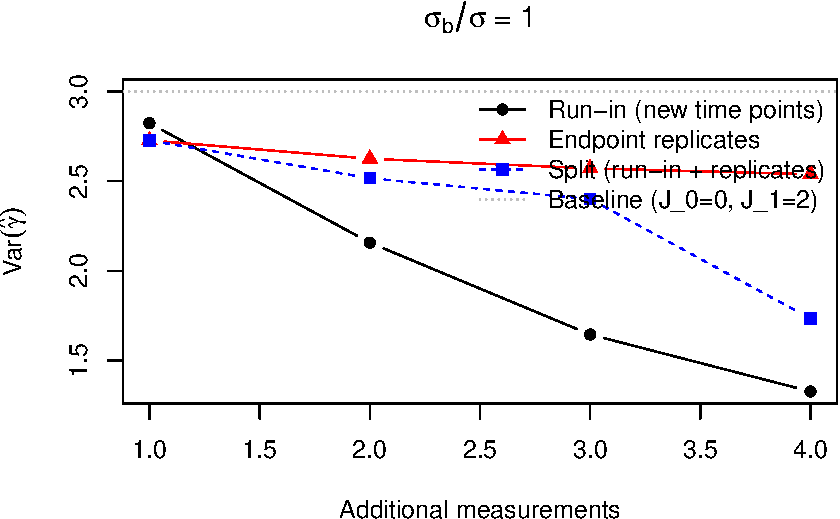
\includegraphics[keepaspectratio,alt={Variance as a function of additional measurements allocated either to run-in (new time points) or endpoint replication (same time point). Baseline: J\_0=0, J\_1=2, \textbackslash sigma\^{}2=1, \textbackslash sigma\_b\^{}2=1.}]{report_files/report_files/figure-latex/rep_vs_runin-1.pdf}}
\caption{Variance as a function of additional measurements allocated
either to run-in (new time points) or endpoint replication (same time
point). Baseline: \(J_0=0\), \(J_1=2\), \(\sigma^2=1\),
\(\sigma_b^2=1\).}
\end{figure}

When \(\sigma_b / \sigma \ge 1\), run-in observations at new time points
outperform endpoint replicates because they provide information about
the individual slope \(b_i\), not just measurement-error reduction. When
\(\sigma_b / \sigma < 1\), endpoint replication can be competitive
because measurement error is the dominant source of variance.

\subsection{Combined replication at both
ends}\label{combined-replication-at-both-ends}

Replicating both the baseline and endpoint visits provides symmetric
measurement-error reduction.

\begin{longtable}[]{@{}
  >{\raggedleft\arraybackslash}p{(\linewidth - 6\tabcolsep) * \real{0.2208}}
  >{\raggedleft\arraybackslash}p{(\linewidth - 6\tabcolsep) * \real{0.2597}}
  >{\raggedleft\arraybackslash}p{(\linewidth - 6\tabcolsep) * \real{0.2597}}
  >{\raggedleft\arraybackslash}p{(\linewidth - 6\tabcolsep) * \real{0.2597}}@{}}
\caption{Per-pair variance with baseline and endpoint replication
(\(J_0=0\), \(J_1=2\), \(\sigma^2=1\),
\(\sigma_b^2=1\)).}\tabularnewline
\toprule\noalign{}
\begin{minipage}[b]{\linewidth}\raggedleft
\(n_{\text{pre}}\)
\end{minipage} & \begin{minipage}[b]{\linewidth}\raggedleft
\(n_{\text{post}}=1\)
\end{minipage} & \begin{minipage}[b]{\linewidth}\raggedleft
\(n_{\text{post}}=2\)
\end{minipage} & \begin{minipage}[b]{\linewidth}\raggedleft
\(n_{\text{post}}=3\)
\end{minipage} \\
\midrule\noalign{}
\endfirsthead
\toprule\noalign{}
\begin{minipage}[b]{\linewidth}\raggedleft
\(n_{\text{pre}}\)
\end{minipage} & \begin{minipage}[b]{\linewidth}\raggedleft
\(n_{\text{post}}=1\)
\end{minipage} & \begin{minipage}[b]{\linewidth}\raggedleft
\(n_{\text{post}}=2\)
\end{minipage} & \begin{minipage}[b]{\linewidth}\raggedleft
\(n_{\text{post}}=3\)
\end{minipage} \\
\midrule\noalign{}
\endhead
\bottomrule\noalign{}
\endlastfoot
1 & 3.0000 & 2.7273 & 2.6250 \\
2 & 2.7273 & 2.5000 & 2.4138 \\
3 & 2.6250 & 2.4138 & 2.3333 \\
\end{longtable}

\section{Incorporating dropout}\label{incorporating-dropout}

\subsection{Pattern-mixture approach}\label{pattern-mixture-approach}

Following Frost et al. (\citeproc{ref-frost2008}{2008}) (Section 2.3),
dropout is handled via a pattern-mixture model
(\citeproc{ref-dawson1993}{Dawson and Lagakos 1993};
\citeproc{ref-lu2008}{Lu et al. 2008}). Participants are stratified by
their observed visit pattern, and the overall variance is a weighted
average: \begin{equation}
  N = \frac{1}{\sum_{s} p_s / N_s}
\end{equation} where \(p_s\) is the proportion with pattern \(s\) and
\(N_s\) is the sample size that would be needed if all participants had
pattern \(s\). This approximation treats each stratum independently. Hu
et al. (\citeproc{ref-hu2021}{2021}) derive exact variance formulas
under monotone dropout for the three-component random coefficient
regression model (\(\sigma^2, \sigma_a^2, \sigma_b^2\)), accounting for
the effect of dropout on the estimability of the random slope variance.
Their approach is more rigorous than the pattern-mixture approximation
used here, which is conservative when dropout is informative about the
random slope.

\begin{longtable}[]{@{}rrr@{}}
\caption{Sample size adjusted for dropout via pattern-mixture
(\(J_0=2\), \(J_1=2\), \(J_2=1\), MIRIAD parameters).}\tabularnewline
\toprule\noalign{}
Annual dropout & \(N\) (no dropout) & \(N\) (with dropout) \\
\midrule\noalign{}
\endfirsthead
\toprule\noalign{}
Annual dropout & \(N\) (no dropout) & \(N\) (with dropout) \\
\midrule\noalign{}
\endhead
\bottomrule\noalign{}
\endlastfoot
0.0 & 1 & 1 \\
0.1 & 1 & 2 \\
0.2 & 1 & 2 \\
0.3 & 1 & 2 \\
\end{longtable}

\section{Numerical examples}\label{numerical-examples}

\subsection{AD neuroimaging trial}\label{ad-neuroimaging-trial}

Using MIRIAD parameters (\(\sigma^2 = 0.0025\), \(\sigma_b^2 = 0.9745\),
\(t = 1\) year), compare the optimal allocation for \(J = 4, 5, 6\)
total observations with and without dropout.

\begin{longtable}[]{@{}lrr@{}}
\caption{Top 10 allocations for \(J=5\) observations (MIRIAD parameters,
\(\Delta=0.25\), 90\% power).}\tabularnewline
\toprule\noalign{}
\((J_0, J_1, J_2)\) & \(\mathop{\mathrm{Var}}_1(\hat\gamma)\) & \(N\)
per group \\
\midrule\noalign{}
\endfirsthead
\toprule\noalign{}
\((J_0, J_1, J_2)\) & \(\mathop{\mathrm{Var}}_1(\hat\gamma)\) & \(N\)
per group \\
\midrule\noalign{}
\endhead
\bottomrule\noalign{}
\endlastfoot
(0,3,2) & 0.002302 & 1 \\
(0,2,3) & 0.002302 & 1 \\
(1,2,2) & 0.003558 & 1 \\
(2,3,0) & 0.004601 & 1 \\
(3,2,0) & 0.004604 & 1 \\
(2,2,1) & 0.004939 & 1 \\
(1,3,1) & 0.005140 & 1 \\
(0,4,1) & 0.005240 & 1 \\
(0,1,4) & 0.005250 & 1 \\
(1,1,3) & 0.006104 & 2 \\
\end{longtable}

\section{Discussion}\label{discussion}

\section{Conflict of interest}\label{conflict-of-interest}

The author declares no conflicts of interest.

\section{Funding}\label{funding}

This work received no specific funding.

\section{Data availability statement}\label{data-availability-statement}

The \texttt{runinpower} R package implementing the optimal-allocation
routines (\texttt{allocation.R}, \texttt{replicated.R},
\texttt{design.R}), validation tests, and the shared bibliography across
the four-paper compendium are openly available in the project
repository. Specific paths are listed in the Reproducibility section
below.

\section{Reproducibility}\label{reproducibility}

This manuscript was rendered with R 4.4.x. Principal packages used are
the in-package \texttt{runinpower} source, \texttt{tinytest} (testing
harness), and \texttt{rmarkdown} plus \texttt{bookdown} for the
manuscript build.

\textbf{Random-number generator.} Optimisation results are deterministic
given fixed input parameters. Where Monte Carlo benchmarking is
reported, the driver sets \texttt{set.seed(20260418)} at its entry
point.

\textbf{Data and code availability.} The R package source is at
\texttt{R/}. The companion manuscripts (Papers 1, 2, 4) are at
\texttt{analysis/paper\{1,2,4\}-*/}. The manuscript source and shared
bibliography (\texttt{../references.bib}) are at
\texttt{analysis/paper3-allocation/}.

\section{References}\label{references}

\protect\phantomsection\label{refs}
\begin{CSLReferences}{1}{1}
\bibitem[\citeproctext]{ref-dawson1993}
Dawson, Jeffrey D., and Stephen W. Lagakos. 1993. {``Size and Power of
Two-Sample Tests of Repeated Measures Data.''} \emph{Biometrics} 49 (4):
1022--32.

\bibitem[\citeproctext]{ref-frison1992}
Frison, Lars, and Stuart J. Pocock. 1992. {``Repeated Measures in
Clinical Trials: Analysis Using Mean Summary Statistics and Its
Implications for Design.''} \emph{Statistics in Medicine} 11 (13):
1685--704. \url{https://doi.org/10.1002/sim.4780111304}.

\bibitem[\citeproctext]{ref-frost2008}
Frost, Chris, Michael G. Kenward, and Nick C. Fox. 2008. {``Optimizing
the Design of Clinical Trials Where the Outcome Is a Rate. {Can}
Estimating a Baseline Rate in a Run-in Period Increase Efficiency?''}
\emph{Statistics in Medicine} 27 (18): 3717--31.
\url{https://doi.org/10.1002/sim.3280}.

\bibitem[\citeproctext]{ref-galbraith2002}
Galbraith, Sally, and Ian C. Marschner. 2002. {``Guidelines for the
Design of Clinical Trials with Longitudinal Outcomes.''}
\emph{Controlled Clinical Trials} 23 (3): 257--73.
\url{https://doi.org/10.1016/S0197-2456(02)00205-2}.

\bibitem[\citeproctext]{ref-goulet2019}
Goulet, Marc-André, and Denis Cousineau. 2019. {``The Power of
Replicated Measures to Increase Statistical Power.''} \emph{Advances in
Methods and Practices in Psychological Science} 2: 199--213.

\bibitem[\citeproctext]{ref-hu2021}
Hu, Na, Hugh Mackey, and Ronald G. Thomas. 2021. {``Power and Sample
Size for Random Coefficient Regression Models in Randomized Experiments
with Monotone Missing Data.''} \emph{Biometrical Journal} 63: 806--24.
\url{https://doi.org/10.1002/bimj.202000184}.

\bibitem[\citeproctext]{ref-iddi2022}
Iddi, Samuel, and Michael C. Donohue. 2022. {``Power and Sample Size for
Longitudinal Models in {R} -- the Longpower Package and {Shiny} App.''}
\emph{The R Journal} 14 (1): 264--82.
\url{https://journal.r-project.org/articles/RJ-2022-022/}.

\bibitem[\citeproctext]{ref-lu2008}
Lu, Kaifeng, Xiaolei Luo, and Pin-Yen Chen. 2008. {``Sample Size
Estimation for Repeated Measures Analysis in Randomized Clinical Trials
with Missing Data.''} \emph{International Journal of Biostatistics} 4
(1): Article 9. \url{https://doi.org/10.2202/1557-4679.1098}.

\bibitem[\citeproctext]{ref-nash2021}
Nash, Stephen, Katy E. Morgan, Chris Frost, and Amy Mulick. 2021.
{``Power and Sample-Size Calculations for Trials That Compare Slopes
over Time: Introducing the Slopepower Command.''} \emph{The Stata
Journal} 21: 572--601. \url{https://doi.org/10.1177/1536867X211045512}.

\bibitem[\citeproctext]{ref-overall1994}
Overall, John E., and Shannon R. Doyle. 1994. {``Estimating Sample Sizes
for Repeated Measurement Designs.''} \emph{Controlled Clinical Trials}
15 (2): 100--123. \url{https://doi.org/10.1016/0197-2456(94)90015-9}.

\bibitem[\citeproctext]{ref-winkens2007}
Winkens, Bjorn, Gerard J. P. van Breukelen, Hubert J. A. Schouten, and
Martijn P. F. Berger. 2007. {``Randomized Clinical Trial Designs for
Auto-Correlated Longitudinal Data.''} \emph{Statistics in Medicine} 26
(28): 5023--37. \url{https://doi.org/10.1002/sim.2907}.

\bibitem[\citeproctext]{ref-winkens2005}
Winkens, Bjorn, Hubert J. A. Schouten, Gerard J. P. van Breukelen, and
Martijn P. F. Berger. 2005. {``Optimal Time-Points in Clinical Trials
with Linearly Divergent Treatment Effects.''} \emph{Statistics in
Medicine} 24 (24): 3743--56. \url{https://doi.org/10.1002/sim.2370}.

\bibitem[\citeproctext]{ref-yi2002}
Yi, Qilong, and Tony Panzarella. 2002. {``Estimating Sample Size for
Tests on Trends Across Repeated Measurements with Missing Data Based on
the Interaction Term in a Mixed Model.''} \emph{Controlled Clinical
Trials} 23 (5): 481--96.
\url{https://doi.org/10.1016/S0197-2456(02)00228-3}.

\end{CSLReferences}

\vfill

\begin{center}\rule{0.5\linewidth}{0.5pt}\end{center}

\emph{Rendered on 2026-05-11 at 18:41 PDT.}\\
\emph{Source:
\texttt{\textasciitilde{}/prj/res/04-runin-power-analysis/runinpower/analysis/paper3-allocation/report.Rmd}}

\end{document}
